\chapter{Introduction}

Safety critical robot applications require extensive testing or formal verification in order to achieve adequate safe and predictable behaviour.
Even if a program does not control actuators itself and thus cannot directly cause any damage, its output might still be a trigger for dangerous actions involving several actors.
Imagine a medication reminder application running on a service robot which guides a person through the process of medication intake, such as the healthcare robotics project at the University
\begin{wrapfigure}{r}{0.58\textwidth}
  \centering
  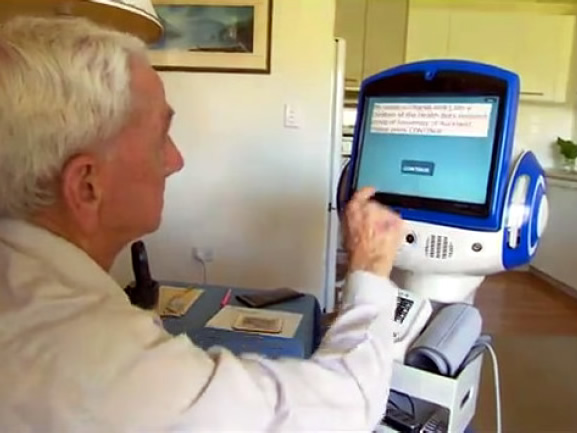
\includegraphics[width=0.56\textwidth]{cafero_being_used}
  \caption{Service robot being used by older person~\cite{robostudio}.}
  \label{fig:cafero_being_used}
\end{wrapfigure}
of Auckland, New Zealand \cite{jayawardena12:_desig}. All interaction is guided by showing textual instructions on a display, and by speech generation. An error in the program logic could cause an already taken medication to be reminded again and may injure a patient with Alzheimer's disease by causing a medication overdose.
Scientists are working on applications such as the medication reminder~\cite{p11:_feasib} which run on mobile robots serving in nursing homes for the elderly. Equipped with a touch display and several external devices such as a blood pressure measurement tool the robots aim to support and entertain the elderly in their daily activities~\cite{jayawardena12:_desig,5649910}.

With service robots coexisting with people and acting within their work\-spa\-ces, coping with reliability and safety issues is essential for trust and acceptance of these robots. In some cases safety certifications based on international standards for functional safety, such as ISO 13482 and IEC 61508, might be even required before robots get released for use or obtain concession for sale.
However, considering functional safety while developing service robots is both complex and difficult; maybe one reason for the absense of safety checks and warranties in the current healthbot versions at the University of Auckland.
But facing the fact that safety requirements for service robots are expected to increase in future, there is a plan of slowly integrating safety functionality into the healthcare robotics project as a next step starting with the concepts introduced in this paper.

The applications for the healthcare robots mentioned above are intended to be developed by healthcare professionals using Robostudio~\cite{robostudio}, a visual programming environment for rapid authoring and customization of complex robot services.
%state machine based processes and a graphical tool for the designing of human robot interaction.
Generally these people don't have profound knowledge of the complex mathematical syntax used for formal temporal logic such as computation tree logic (CTL) or linear temporal logic (LTL). Nevertheless certain safety guarantees must somehow be delivered in order to gain users' trust and to prevent any harm or injuries by the healthcare robots.
In case of the medication reminder mentioned above it might be important to ensure notifications are sent to staff members whenever medication is not taken by the patient, or to avoid duplicate reminders for medications which have already been taken.
So a mechanism is needed for the specification of such safety constraints; one that does not require special or expert knowledge and thus is easy to use for all kind of programmers. A visual language intended to fill this gap is presented in section~\ref{sec:operatorconstraints}.

Unfortunately the supply of an easy-to-use editor for constraint creation doesn't guarantee adequate thinking about sufficent constraints by the developer. Unmotivated or just unexperienced developers may miss important constraints needed in order to achieve a certain safety level.
To support the user in finding significant constraints it might be useful to automatically compute constraint suggestions which make true testimonies about the current designed program. First of all the generated constraints provide an opportunity for the developer to identify reasonable constraints as well as contradictions between constraints and specification. The latter would mean there are errors in the program which lead to undesired constraints. Furthermore once constraints are created and checked for sanity they can be validated after every program change and thus ensure integrity during the development process. In chapter~\ref{chap:automatedconstraintgeneration} we introduce a heuristic for finding reasonable safety constraints based on state machine definitions that describe robots' behaviours.

Both ideas are to be integrated into Robostudio in order to simplify respectively facilitate the use of safety mechanisms for application development for service robots. Thereby a desired safety certification for the healthcare service robots can move closer one step.

This work starts with background information about the healthcare domain, short explanations of common safety mechanisms and insights into related work in chapter~\ref{chap:background}. After the goals are mentioned in chapter~\ref{chap:goals}, the visual formalisms and the automated constraint generation are introduced in chapters~\ref{chap:visualformalisms} and~\ref{chap:automatedconstraintgeneration}.
After a prototype implementation is demonstrated in chapter~\ref{chap:theltlcreatorprototype}, a test scenario is described in chapter~\ref{chap:testscenarioandevaluation} where the presented tools get evaluated.
Chapter~\ref{chap:conclusionandfuturework} gives a short conclusion and an outlook how the work presented in this paper could be continued.

%Once such constraints are defined, they determine the grade of safety coverage. Unfortunately, the program may still contain errors if there is at least one significant constraint missed out. To support the user in finding such ones the tool could furthermore automatically compute suggestions for possible constraints based on the designed statemachine. These are displayed to the programmer and may help him identifying reasonable constraints as well as contradictions between program and specification.

%Our approach presented in this paper has a special focus on the healtcare domain.


%Dieses beispiel ist eine Anwendung eines umfangreichen Healthcare-Projekts, an dem im robotics lab der Universit�t von Auckland gearbeitet wird. Die zustansbasierten Anwendungen laufen auf Cafero, einem mit blutdruckmessger�t und anderen tools austestatteten mobilen Roboter mit Touchdisplay.
%Die einzelnen Anwendungen werden von Healthcare-Professionals mit dem Tool Robostudio [cite] entwickelt, das eine graphische oberfl�sche zur modellierung von zustandsmaschinen externen services und  bietet.
%Allerdings haben diese not to have profound knowledge of the complex mathematical syntax used for formal verification methods such as computation tree logic (CTL) or linear temporal logic (LTL)).
%Dennoch m�chte man gegen�ber den Patienten, die von solchen Robotern gepflegt werden, ein gewisses Level an Sicherheit gew�hrleisten k�nnen. Beispielsweise soll in obigem Beispiel sichergestellt werden k�nnen, dass ein Medikament nach der Einnahme nicht erneut in einer Erinnerung auftaucht, oder dass bei Nichteinnahme ein Mitarbeiter benachrichtigt wird.
%Dazu bedarf es allerdings Mechanismen zur spezifizierung solcher Sicherheitseigenschaften, die f�r den Programmentwickler zug�nglich und einfach (am besten ohne spezialwissen) zu benutzen sind.


%Among others robots are alredy used in elderly care centers for healthcare purpose.

% -->

%Robostudio (oder healthcare applikation) soll irgendwann Sicherheitszertifizierung bekommen (erklaeren warum). Daher ist es wichtig, sicherheitsmechanismen zur verfuegung zu stellen. Einen kleinen Schritt in diese Richtung m�chten wir mit dieser Arbeit machen...
%Anwender kommen aus verschiedenen Domaenen => need of easy-to-use safety functionality


%Aiming for safe and reliable robots,
%IEC 61508 certification. It contributes to reducing costs and development time when creating highly-dependable and safe robots.



%Glossary IEC 61508
%IEC 61508 is an international standard, produced in 2000 by the IEC, for the realisation of functional safety in devices utilising computer technology. Functional safety differs from inherent safety in that its goal is to reduce risk to permissible levels using active techniques, rather than passive techniques. IEC 61508 specifies guidelines for developing safety-related hardware and software, and management techniques for development processes to ensure accurate designs and implementations.
% <--